\begin{frame}{Parameterized Policies}
\begin{itemize}
    \item For the purpose of this lecture we will focus on policies parameterized by Neural Nets.
    \item For \textbf{Discrete action spaces}, the network takes the state representation as the input and outputs the probabilities of taking each action (Softmax Policy). Analogus to classification in Supervised Learning.
\end{itemize}
\begin{center}
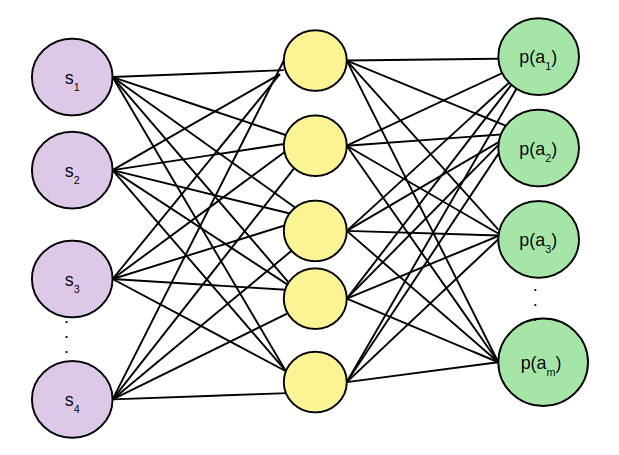
\includegraphics[scale=0.3]{img/discaction.png}
\end{center}
\end{frame}
\begin{frame}{Parameterized Policies}
\begin{itemize}
    \item In case of \textbf{Continuous action spaces}, we assume our policy to be gaussian and the network takes the state as input and outputs the mean and diagonal covariance of the distribution. Analogus to regression in Supervised Learning.
\end{itemize}
\begin{center}
    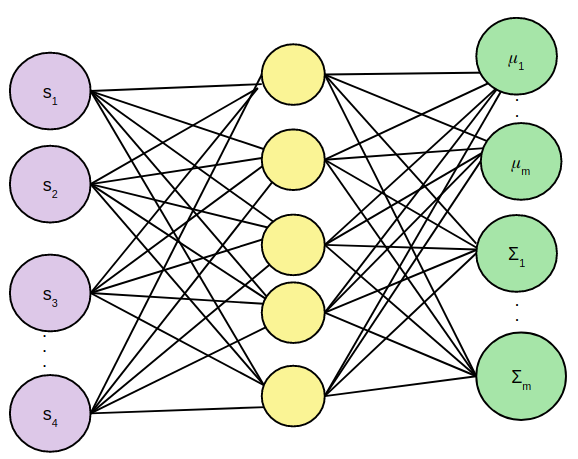
\includegraphics[scale=0.3]{img/contaction.png}

\end{center}
\end{frame}
\begin{frame}{Policy Optimization Objective}
\begin{columns}
\column{0.45\textwidth}
    \begin{itemize}
        \item[] $s_0 \sim \mu(s_0)$
        \item[] $a_0 \sim \pi(a_0|s_0;\theta)$
        \item[] $s_1 \sim \mathbb{P}(s_1|s_0, a_0)$
        \item[] $r_0 \sim \mathbb{R}(s_0, a_0, s_1)$
        \item[] $a_1 \sim \pi(a_1|s_1;\theta)$
        \item[] $s_2 \sim \mathbb{P}(s_2|s_1, a_1)$
        \item[] $r_1 \sim \mathbb{R}(s_1, a_1, s_2)$
        \item[] ...
        \item[] $a_{T-1} \sim \pi(a_{T-1}|s_{T-1};\theta)$
        \item[] $s_T \sim \mathbb{P}(s_T|s_{T-1}, a_{T-1})$
        \item[] $r_{T-1} \sim \mathbb{R}(s_{T-1}, a_{T-1}, s_{T})$
    \end{itemize}
\column{0.55\textwidth}
    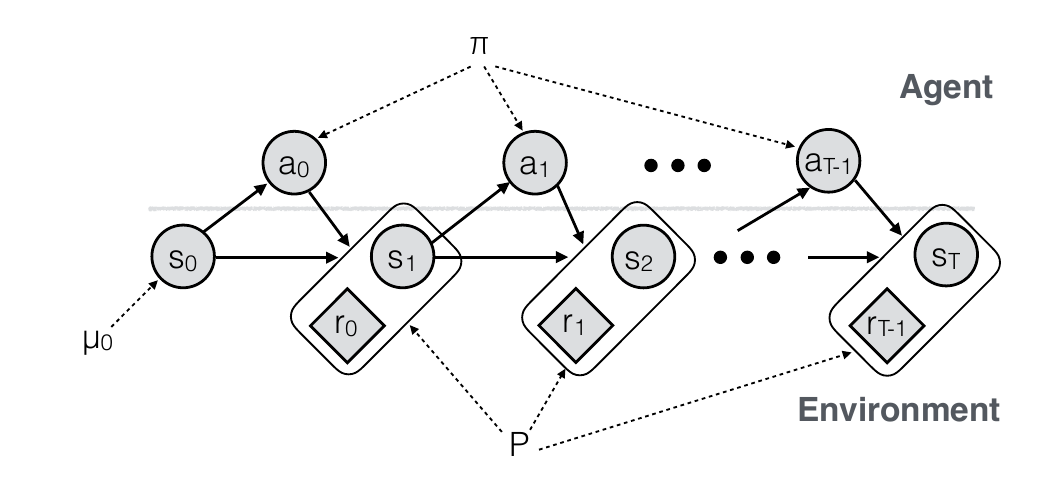
\includegraphics[scale=0.18]{img/trajvis.png}
\end{columns}
\footnotetext[1]{Image from John Schulman slides on Policy Gradients.}
\end{frame}
\begin{frame}{Policy Optimization Objective}
\textbf{Objective Function}
\newline
maximize $\eta(\pi_{\theta})$
\newline
where
\begin{equation}
    \begin{split}
        \eta(\pi_{\theta}) & = \mathop{\mathbb{E}_{\tau}}[r_0 + \gamma r_1 + \gamma^2 r_2 + ... + \gamma^{T-1}r_{T-1}|\pi_{\theta}]\\
        & = \mathop{\mathbb{E}_{\tau}}[R(\tau)|\pi_{\theta}]
    \end{split}
\end{equation}
and $\tau$ denotes a trajectory $(s_0,a_0,r_0,s_1,a_1,r_1,...,s_T, a_{T-1}, r_{T-1})$
\newline
\textbf{Intuition}
\newline
By maximizing this objective function we:
\begin{itemize}
    \item Make the good trajectories more probable.
    \item By making good trajectories more probable we also make good actions more probable.
\end{itemize}
\end{frame}
\begin{frame}{Solving the Optimization Problem}
\begin{itemize}
    \item Note that our objective function is not a direct function of policy parameters $\theta$
    \item To optimize the function using gradient based methods we need a way to estimate the gradients of the objective with respect to $\theta$
    \item \textbf{Score function gradient estimator}  is used for this purpose.
\end{itemize}
    
\end{frame}

\begin{frame}{Score Function Gradient Estimator}
\begin{itemize}
    \item Consider an optimization problem of maximizing $\mathop{\mathbb{E}}_{x \sim p(x|\theta)}[f(x)]$ with respect to $\theta$
\end{itemize}
\begin{equation}
    \begin{split}
            \nabla_{\theta}\mathop{\mathbb{E}_x}[f(x)] & = \nabla_{\theta} \sum_x p(x|\theta)f(x)\\
    & = \sum_x \nabla_{\theta}p(x|\theta)f(x)\\
    & = \sum_x p(x|\theta)\frac{\nabla_{\theta}p(x|\theta)}{p(x|\theta)}f(x)\\
    & = \sum_x p(x|\theta)\nabla_{\theta}\log p(x|\theta)f(x)\\
    & = \mathop{\mathbb{E}_x}[f(x) \nabla_{\theta}\log p(x|\theta)]\\
    \end{split}
\end{equation}
    
\end{frame}
\begin{frame}{Score Function Gradient Estimator}
\textbf{Intuition}
\newline 
Lets denote the score function estimator as $g_i = f(x_i)\nabla_{\theta} \log p(x_i|\theta)$
\begin{itemize}
    \item Let $f(x)$ denotes how good a sample $x$ is.
    \item Moving in the direction of $g$ pushes the probability of $x$ in the proportion of how good it is ($f(x)$).
    \item A sample which leads to a small value of $f(x)$ will lead to adjustment of parameters $\theta$ such that its log probability is reduced as compared to the samples with higher $f(x)$ and vice versa.
    \item  \textbf{$f(x)$ need not be a continuous or differentiable function}.
\end{itemize}
    
\end{frame}
\begin{frame}{Score Function Gradient Estimator}
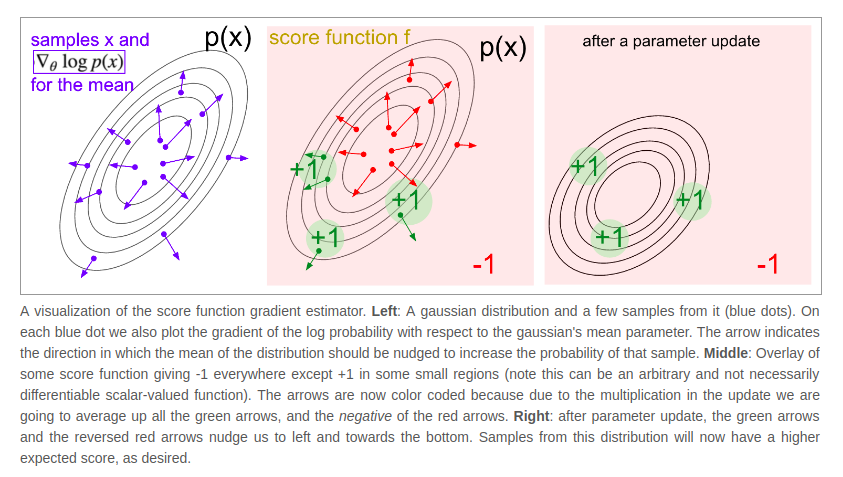
\includegraphics[scale = 0.4]{img/scoreFunction.png}
 \footnotetext[1]{Image from Andrej Karpathy's blog\\ (https://karpathy.github.io/2016/05/31/rl/)}
\end{frame}
\begin{frame}{Score Function Gradient Estimator for Policies}
\begin{itemize}
    \item Remember our objective function was: $\max_{\theta}$ $\mathop{\mathbb{E}_{\tau}}[R(\tau)]$
    \item The random variable $x$ in this case is the trajectory $\tau$ denoted by $(s_0,a_0,r_0,s_1,a_1,r_1,...,s_T, a_{T-1}, r_{T-1})$
    \item And the function $f$ is the total cumulative reward. $f(\tau) = R(\tau) = \sum_t \gamma^tr_t$
    \item The probability of the trajectory can be computed as:
\end{itemize}
\begin{equation*}
    \begin{split}
        &p(\tau) = \mu(s_0)\pi(a_0|s_0;\theta)\mathbb{P}(s_1|s_0,a_0)\pi(a_1|s_1;\theta)\mathbb{P}(s_2|s_1,a_1)...\\
        &p(\tau)= \mu(s_0)\prod_{t=0}^{T-1} \pi(a_t|s_t;\theta)\mathbb{P}(s_{t+1}|s_t,a_t)\\
    &\log p(\tau) = \log \mu(s_0) + \sum_{t=0}^{T-1}\log\pi(a_t|s_t;\theta) + \sum_{t=0}^{T-1}\log \mathbb{P}(s_{t+1}|s_t,a_t)
    \end{split}
\end{equation*}

    
\end{frame}
\begin{frame}{Score Function Gradient Estimator for Policies}
    \begin{equation*}
        \begin{split}
            & \nabla_\theta \log p(\tau) = \nabla_\theta \sum_{t=0}^{T-1}\log\pi(a_t|s_t;\theta) \\
            & \nabla_\theta \mathop{\mathbb{E}_\tau}[R] = \mathop{\mathbb{E}_\tau}[R \nabla_\theta \sum_{t=0}^{T-1}\log\pi(a_t|s_t;\theta)]\\
            & \nabla_\theta \mathop{\mathbb{E}_\tau}[R] = \mathop{\mathbb{E}_\tau}[(\sum_{t=0}^{T-1} \gamma^tr_t)( \nabla_\theta \sum_{t=0}^{T-1}\log\pi(a_t|s_t;\theta))]
        \end{split}
    \end{equation*}
    \textbf{Intuition}: Good trajectories i.e. the trajectories with higher values of $R$ will serve as supervised examples like in the case of classification or regression.
\end{frame}

\begin{frame}{Score Function Gradient Estimator for Policies}
    \begin{itemize}
        \item A slightly better estimate can be obtained by rearranging the terms in the expression above and we obtain:
        $\nabla_\theta \mathop{\mathbb{E}_\tau}[R] = \mathop{\mathbb{E}_\tau}[ \nabla_\theta \sum_{t=0}^{T-1}\log\pi(a_t|s_t;\theta)\sum_{t' = t}^{T-1} \gamma^{t'} r_{t'}]$
        \item The second term in the expression can be interpreted as an estimate of action value function (Q)
        $\nabla_\theta \mathop{\mathbb{E}_\tau}[R] = \mathop{\mathbb{E}_\tau}[\nabla_\theta \sum_{t=0}^{T-1}\log\pi(a_t|s_t;\theta)Q(s_t,a_t)]$
    \end{itemize}
\end{frame}
\begin{frame}{Practical Implementation with Autodiff}
\begin{itemize}
    \item Collect $n$ different trajectories $\tau_i = (s_0^i,a_0^i,r_0^i,s_1^i,a_1^i,r_1^i,...,s_T^i, a_{T-1}^i, r_{T-1}^i)$
    \item For each trajectory $\tau_i$ compute Q value estimates
    $Q(s_t^i, a_t^i) = \sum_{t' = t}^{T-1}\gamma^{t'}r_{t'}^i$
    \item The log probabilities can be obtained from the output of neural network $f$.
    \begin{itemize}
        \item For Discrete Action Spaces:
        $\log\pi(a_t^i|s_t^i;\theta) = \log f(s_t^i;\theta)$
        \item For Continuous Action Spaces:
        \begin{equation*}
            \begin{split}
               &\mu_t^i, \sigma_t^i = f(s_t;\theta)\\
                &\log\pi(a_t^i|s_t^i;\theta) = \frac{-(a_t^i-\mu_t^i)^2}{2\sigma_t^{i2}} - \frac{1}{2}\log(2\pi^k\sigma_t^i)
            \end{split}
        \end{equation*}
    \end{itemize}
\end{itemize}

\end{frame}
\begin{frame}{Practical Implementation with Autodiff}
    \begin{itemize}
    \item Define the surrogate loss as:
    $L_{surr}(\theta) = -\frac{\sum_{i = 1}^n \sum_{t=0}^{T-1}Q(s_t^i,a_t^i)\log\pi(a_t|s_t;\theta))}{n}$
    \item Find policy gradient estimate: $g(\theta) = \nabla_{\theta}L_{surr}(\theta)$
    \begin{itemize}
        \item Pytorch: loss.backward()
        \item Tensorflow : tf.train.Optimizer().minimize(loss)
    \end{itemize}
    \item Plug $g(\theta)$ in your favourite optimizer SGD/ ADAM
    \item This algorithm is called REINFORCE or Vanilla Policy Gradient
\end{itemize}
\end{frame}
\begin{frame}{Collecting Trajectories}
    \begin{itemize}
        \item[] Initialize sets $S, A, R, P$ for storing states, actions, rewards and neural network outputs.
        \item[] Sample initial state $s_0$ from environment $E$
        \item[] t = 0
        \item[] \textbf{Repeat} till episode \textbf{terminates}
        \begin{itemize}
            \item[] Sample action $a_t$ from $\pi(a_t|s_t,\theta)$ defined using the outputs of neural network $f(s_t)$. (Multinomial Distribution for discrete case and Gaussian for continuous)
            \item[] Execute action $a_t$ in environment $E$ and obtain reward $r_t$ and new state $s_{t+1}$
            \item[] Store $s_t, a_t, r_t, f(s_t)$ in the sets $S, A, R, P$
            \item[] t := t+1
        \end{itemize}
    \end{itemize}
\end{frame}
\begin{frame}{REINFORCE Algorithm}
    \begin{itemize}
        \item[] Initialize policy parameters $\theta$
        \item[] \textbf{for} iteration = 1,2... \textbf{do} 
        \begin{itemize}
            \item[] Collect a set of trajectories using current policy $\pi$.
            \item[] At each time step for each trajectory compute the approximate Q value as: $Q(s_t^i, a_t^i) = \sum_{t' = t}^{T-1}\gamma^{t'}r_{t'}^i$
            \item[] Compute the log probabilities $\log\pi(a_t|s_t;\theta)$ using the output of the neural net.
            \item[] Compute the surrogate loss using log probabilities and Q values.
            \item[] Compute the gradient $g(\theta)$  of the loss function and update the parameters of policy: For eg. SGD Update: $\theta = \theta - \alpha g(\theta)$
        \end{itemize}
        \item[] \textbf{end for}
    \end{itemize}
\end{frame}
